\subsection{Introducción y descripción del algoritmo}
\par En este ejercicio se nos pide implementar una heurística constructiva golosa para resolver el juego.

\par El algoritmo goloso se basa en priorizar ciertos valores del grafo para recorrerlo. En este caso usamos la distancia entre los nodos y buscamos siempre el nodo válido más cercano para saltar a el.
	 	
\par La idea intuitiva es que minimizando la distancia entre cada salto de nodo a nodo se puede llegar a encontrar la mejor solución, cosa que en general no vale. 
	La ventaja es que es fácil de implementar y tiene complejidad polinomial.

\subsection{Idea general del algoritmo}

\par Hay dos tipos de nodos: gimnasios y paradas. Un jugador puede ir de un nodo a cualquier otro que no haya visitado antes. Por lo que solo nos manejaremos con una lista de todos los nodos del grafo . Entre dos nodos cualesquiera existe una distancia, que calcuaremos al inicio. También es importante notar que para ir a un nodo de tipo gimnasio se debe contar con al menos la cantidad de pociones necesarias para vencerlo. Pero al comenzar el jugador no cuenta con ninguna, por lo que el primer nodo ha visitar siempre debe ser uno del tipo parada.

\par Aclarados estos detalles, retomaremos el ejemplo mostrado en la descripción general del problema (figura \ref{fig: descripcion_ejemplo_entrada}), veremos las distancias entre estos nodos y analizaremos el funcionamiento del algoritmo sobre este caso en particular.

\begin{table}[h]
	\centering
	\begin{tabular}{|>{\centering\arraybackslash}p{2cm}|>{\centering\arraybackslash}p{2cm}|>{\centering\arraybackslash}p{2cm}|>{\centering\arraybackslash}p{2cm}|>{\centering\arraybackslash}p{2cm}|}
		\hline
		   & \textbf{G1} & \textbf{G2} & \textbf{P1} & \textbf{P2} \\ \hline
		\textbf{G1} & \cellcolor{gray} & 1.41421 & 2.82842 & 2 \\ \hline
		\textbf{G2} & 1.41421 & \cellcolor{gray} & 1.41421 & 1.41421 \\ \hline
		\textbf{P1} & 2.82842 & 1.41421 & \cellcolor{gray} & 2 \\ \hline
		\textbf{P2} & 2 & 1.41421 & 2 & \cellcolor{gray} \\
		\hline
	\end{tabular}
	\caption{Distancias entre los nodos del caso de ejemplo.}
	\label{fig: ejercicio1_ejemplo_distancias}
\end{table}

\par El algoritmo se basa en recorrer nodo por nodo siempre yendo al vecino más cercano, priorizando los nodos gimnasio si tiene las pociones necesarias para ir a el. Es decir, si puede ir a un nodo gimnasio y a un nodo parada, va a ir al nodo gimnasio. En otro caso va a una parada a buscar más pociones.
\par Al tomar este ejemplo de entrada, el algoritmo comenzará parándose sobre algún nodo \textit{i} del tipo parada (en particular, nos paramos en la pokeparada más cercana al primer gimnasio de la entrada) y calculará el camino goloso partiendo desde él. En el ejemplo, comienza por el nodo \textit{P2}, ya que es la parada más cercana al primer gimnasio \textit{G1}.

\begin{figure}[H]
    \begin{subfigure}[b]{0.49\textwidth}
        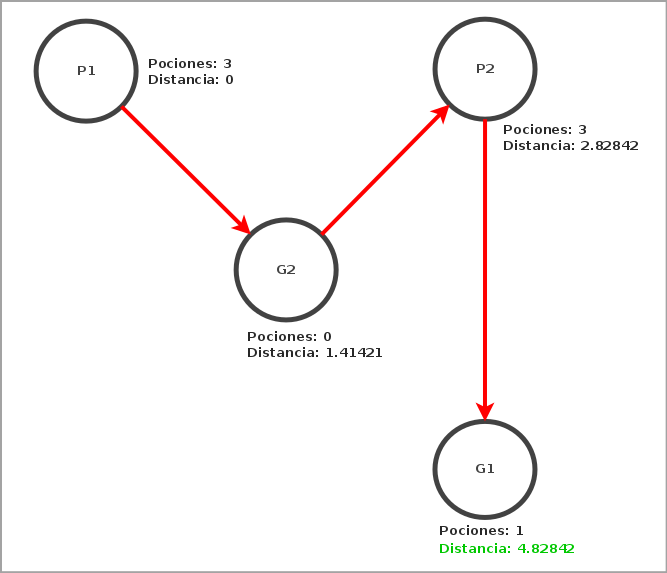
\includegraphics[width=\linewidth]{img/ejercicio2/ejercicio1_ejemplo_camino1_2.png}
        \caption{Camino exacto.}
        \label{fig: ejercicio1_ejemplo_camino1_2}
    \end{subfigure}
    \begin{subfigure}[b]{0.49\textwidth}
        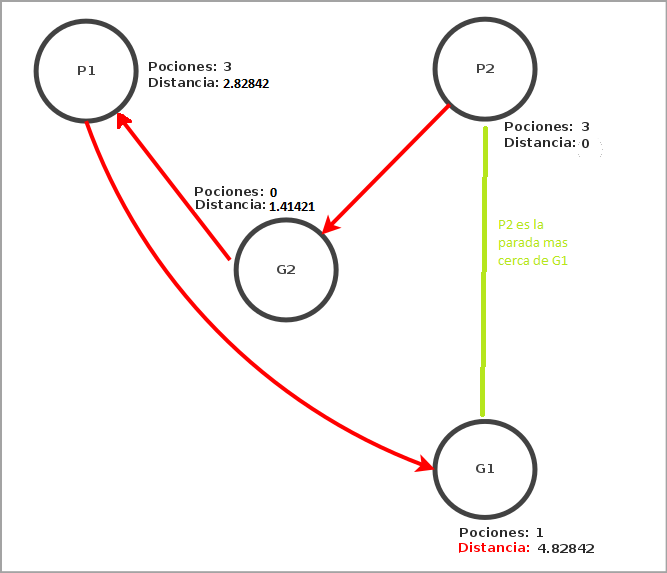
\includegraphics[width=\linewidth]{img/ejercicio2/ejercicio1_ejemplo_camino1_4.png}
        \caption{Camino con algoritmo goloso.}
        \label{fig: ejercicio1_ejemplo_camino1_4}
    \end{subfigure}
    \caption{Camino exacto calculado con backtracking y camino goloso}
    \label{fig: ejercicio1_ejemplo_caminos1}
\end{figure}


\subsection{Explicación del algoritmo}

\par Para nuestro algoritmo goloso tenemos la matriz de distancias del grafo con los nodos que nos pasaron en la entrada


\par La función que calcula el camino goloso recibe los siguientes parámetros:
\begin{itemize}
\item distancias: Es una matriz de distancias ya calculadas a partir de la entrada.
\item gimnasios\_costo : Es un vector que en cada índice $i$ tiene la cantidad de pociones que cuesta matar al gimnasio $i$
\item gimnasios\_totales : Tiene la cantidad total de gimnasios pasador por parámetro.
\end{itemize}
\par El algoritmo es iterativo y tiene la siguiente estructura:

\begin{itemize}
	\item Primero calcula la pokeparada más cercana al primer gimnasio de la entrada y la guarda como el primer nodo a recorrer así como el primer nodo de la solución.
	\item Luego entra en un ciclo que dura mientras la cantidad de gimnasios que recorrimos sea menor a la cantidad total de gimnasios.
	\item Dentro de este ciclo principal se entra en otro ciclo que itera sobre todos los gimnasios para tomar el gimnasio más cercano al nodo actual. Se va tomar el gimnasio más cercano tal que no se haya recorrido y se tengan las pociones necesarias para poder matarlo.
	\item Al salir del ciclo secundario anterior, el algoritmo se fija si encontró algún nodo gimnasio para tomar como el siguiente. En el caso de que no lo haya encontrado hay que iterar de forma similar para encontrar la pokeparada más cercana y sumar las pociones, si no encuentra pokeparada entonces no hay solución al problema y se sale del ciclo principal.
	\par Si encontró un gimnasio se restan las pociones gastadas para matarlo y se suma $uno$ en el contador de gimnasios recorridos. 
\par Por último agrega el nodo que haya encontrado al camino solución.
	\item Una vez afuera del ciclo principal el algoritmo chequea si se recorrieron todos los gimnasios. En caso afirmativo simplemente itera sobre el camino para calcular la distancia recorrida y devolverla. En el otro caso se devuelve un $-1$, ya que no se pudieron matar todos los gimnasios.
\end{itemize}

\medskip

\SetAlgoLined
\SetKwProg{Fn}{Function}{:}{EndFunction}
\begin{algorithm}[H]
	\label{algo: ejercicio2_pseudocodigo}
	\Fn{camino\_goloso(distancias : Matriz(int)), gimnasios\_costo : vector(int), gimnasios\_totales : int}{
		$solucion\_res :$ vector(int)	
		\BlankLine
		$gimnasios\_recorridos \gets$ 0	
		\BlankLine	
		$pocionesActuales \gets$ 0
		\BlankLine
		$distancia\_res \gets 0$
		\BlankLine
		$nodo\_actual \gets $ PokeParadamásCercana(primer gimnasio) \Comment{$O(m) $}
		\BlankLine
		solucion\_res.push(nodo\_actual);
		\BlankLine
		\While{gimnasios\_recorridos $<$ gimnasios\_totales} { 
			\BlankLine
			$gimnasio\_cercano \gets$ -1
			\BlankLine
			\For{gym\_i $<$ gimnasios\_totales; gym\_i++} {
		\BlankLine
		$minimo \gets$ $\infty$
\BlankLine
		\If{ minimo $>$ distancias[gym\_i][nodo\_actual]
           	$\&$    pocionesActuales $\geq$ gimnasios\_costo[gym\_i]) 
             $\&$  NoLoRecorri(gym\_i)}
              {		\BlankLine
			$minimo \gets$ distancias[gym\_i][nodo\_actual]		\BlankLine
                $gimnasiocercano \gets$ gym\_i 		\BlankLine
              }		\BlankLine

			}		\BlankLine		\BlankLine
		
	\If{No encontr\'e gimnasio para matar}{		\BlankLine

       \If{No hay más pokeparadas}{ 		\BlankLine
          break;
        } 			
	       \Else {$nodoActual \gets$ pokeparadamásCercana(nodo\_actual)
			\BlankLine
          $pocionesActuales \gets$ pocionesActuales + 3
	
        }		\BlankLine
      }		\BlankLine
	\Else{ %mato el gimnasio!		
		\BlankLine
        $gimnasios\_recorridos \gets gimnasios\_recorridos + 1$		\BlankLine
        $nodoActual \gets$ gimnasiocercano		\BlankLine
       $ pocionesActuales \gets pocionesActuales - gimnasios\_costo[nodoActual]$		\BlankLine
      }		\BlankLine
      $solucion\_res.push(nodoActual+1)$		\BlankLine
    }	\BlankLine

    \If{gimnasios\_recorridos $<$ gimnasios\_totales} {		\BlankLine		\BlankLine
     %-distancia invalida
      distancia\_res = -1;
    } \Else {		\BlankLine
      $distancia\_res \gets$ CalcularDistancia(solucion\_res)
      }		\BlankLine
		\BlankLine
	return solucion\_res, distancia\_res
}
	

\end{algorithm}



\subsection{Análisis de complejidad}

\par Para analizar la complejidad del algoritmo y su implementación debemos definir ciertos conceptos y parámetros:

\begin{itemize}
	\item \textbf{n}: Cantidad de nodos del tipo gimnasio.
	\item \textbf{m}: Cantidad de nodos del tipo parada.
	\item \textbf{k}: Capacidad de la mochila del jugador.
\end{itemize}



\begin{itemize}
	\item Buscar la pokeparada más cercana al primer gimnasio consiste en un loop que itera sobre las pokeparadas y se queda con la más cercana, eso cuesta O($m$)
	\item El loop principal puede llegar a iterar todos los nodos del grafo, O($n + m$)
	\item Luego viene el loop anidado sobre el anterior e itera sobre los gimnasios, cuesta O($n$). 
	\item En caso de no haber encontrado gimnasio busca pokeparada más cercana, O($m$). Esto es dentro del loop principal , pero fuera del anterior.
	\item Sobre el final, ya fuera de los loops, se itera sobre el camino que quedó para sacar la distancia total, cuesta O($m + n$)
\end{itemize}

\par Vemos que en total todo cuesta O($m$ $+$ $(m+n)^2$ $+$ $m + n$) = O(\textit{max}($m^2, n^2, m*n$)). Vemos más en detalle esta cota:

\begin{equation}
	max(m^2, n^2, m*n)
\end{equation}
tenemos
\begin{equation}
	si\ |m| > |n| \Rightarrow max(m^2, n^2, m*n) = m^2
\end{equation}
\begin{equation}
	si\ |m| < |n| \Rightarrow max(m^2, n^2, m*n) = n^2
\end{equation}
\begin{equation}
	si\ |m| = |n| \Rightarrow max(m^2, n^2, m*n) = m^2 = n^2
\end{equation}
Entonces podemos decir que 
\begin{equation}
	max(m^2, n^2, m*n) = max(m^2, n^2)
\end{equation}

\par De esta manera podemos concluir que la complejidad total del algoritmo es \textbf{O($max(m^2, n^2)$)}.

\subsection{La solución no siempre es la mejor}
	En las imágenes siguientes, la doble flecha negra indica la distancia entre los nodos, y la flecha roja el camino elejido:
\begin{figure}[H]
    \begin{subfigure}[b]{0.49\textwidth}
        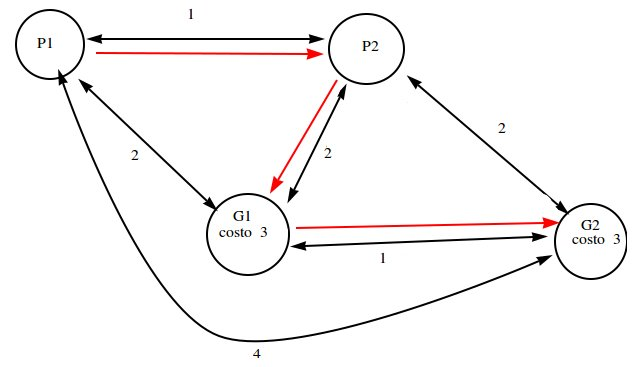
\includegraphics[width=\linewidth]{img/ejercicio2/exacto.jpg}
        \caption{Camino exacto.}
        \label{fig: ejercicio1_ejemplo_camino1_2}
    \end{subfigure}
    \begin{subfigure}[b]{0.49\textwidth}
        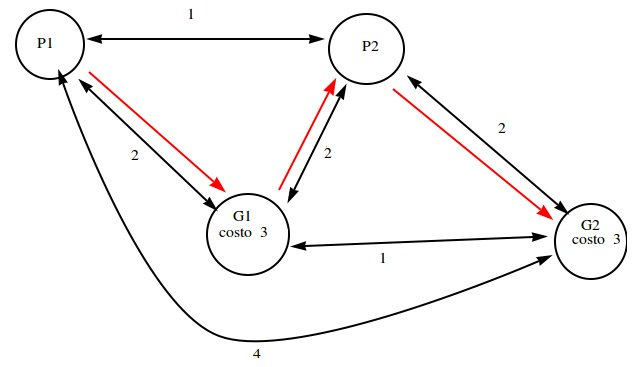
\includegraphics[width=\linewidth]{img/ejercicio2/goloso_malo.jpg}
        \caption{Camino con algoritmo goloso.}
        \label{fig: ejercicio1_ejemplo_camino1_4}
    \end{subfigure}
    \caption{Camino exacto calculado con backtracking y camino goloso}
    \label{fig: ejercicio1_ejemplo_caminos1}
\end{figure}

Como se ve, en el camino exacto la distancia total es $4$, mientras que en el goloso es $6$. 
Esto es en parte a que el goloso empieza en una pokeparada definida y además solo optimiza la distancia localmente, tal vez perdiendo una mejor arista para tomar en otro nodo no vecino al actual.

\subsection{Experimentación}
%	La complejidad del algoritmo es O(\textit{max}($m^2, n^2, m*n$)). Por lo tanto mostramos dos graficos, uno variando la cantidad de gimnasios y otro variando la cantidad de pokeparadas, de 0 a 10:
%	\begin{figure}[H]
%    \begin{subfigure}[b]{0.49\textwidth}
%        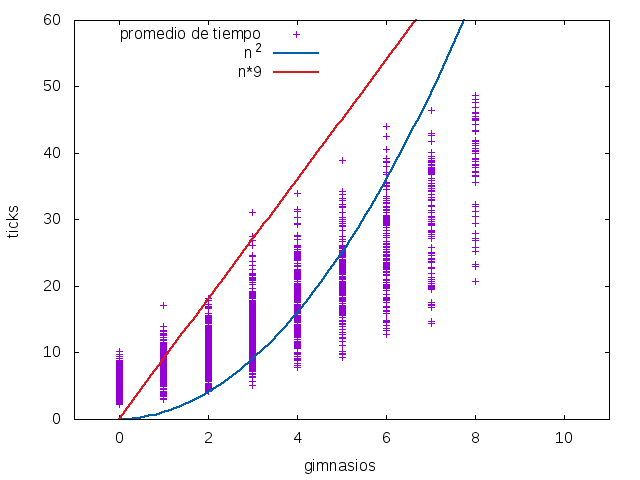
\includegraphics[width=\linewidth]{img/ejercicio2/salidaN.png}
%        \caption{Grafico variando los gimnasios.}
%        \label{fig: ejercicio1_ejemplo_camino1_2}
%    \end{subfigure}
%    \begin{subfigure}[b]{0.49\textwidth}
%        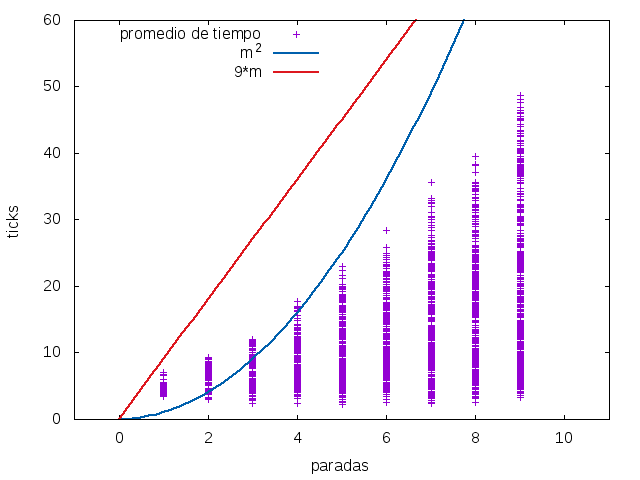
\includegraphics[width=\linewidth]{img/ejercicio2/salidaM.png}
%        \caption{Grafico variando las pokeparadas.}
%        \label{fig: ejercicio1_ejemplo_camino1_4}
%    \end{subfigure}
%    \label{fig: ejercicio1_ejemplo_caminos1}
%\end{figure}
%
%Por cada $x$ del dominio tenemos 10 cruces, que son los tiempo de ejecución habiendo fijado ese x y moviendo la otra variable. Es decir, si en el gráfico de gimnasios tomamos $gimnasios = 2$, tenemos los tiempo de ejecución de $( gimnasios = 2, paradas = 0...9) $. 
%
%\par Como la complejidad viene en función de un máximo, graficamos cada candidato a máximo y vemos que cada uno es más grande que los tiempos de ejecución.
%\par En el caso de O$(n*m)$ graficamos la funciòn $9 * m$ o $n * 9$, que es el máximo valor que puede llegar a tomar en nuestro muestreo.
%
%\par En ambos casos se ve como la complejidad tiene una tendencia mayor a los tiempos de ejecución.
%\\
%En el siguiente gráfico variamos la mochila fijando las otras variables:
%	\begin{figure}[H]
%    \begin{subfigure}[b]{0.49\textwidth}
%        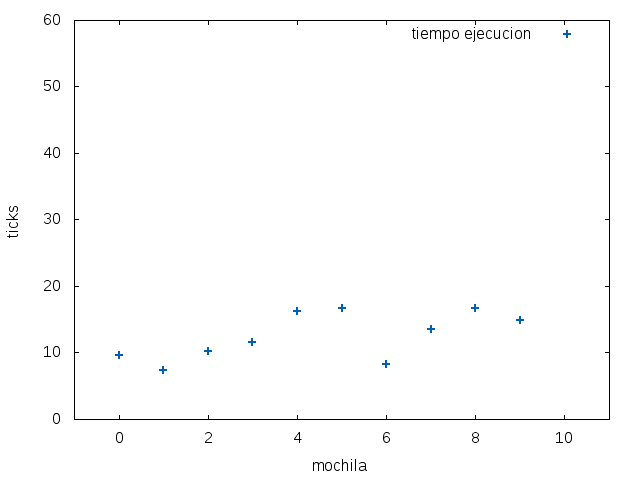
\includegraphics[width=\linewidth]{img/ejercicio2/salidaMochifijadaM.png}
%        \caption{Grafico variando las mochilas.}
%        \label{fig: ejercicio1_ejemplo_camino1_2}
%    \end{subfigure}
%    
%    \label{fig: ejercicio1_ejemplo_caminos1}
%\end{figure}
%
%En este caso la función no tiene una tendencia a crecer. Esto es lo que se esperaba, ya que la complejidad no depende de la amplitud de la mochila, por lo tanto los tiempos de ejecución deberían mantenerse en orden constante al variar la mochila.


%\begin{figure}[H]
%  \begin{center}
%    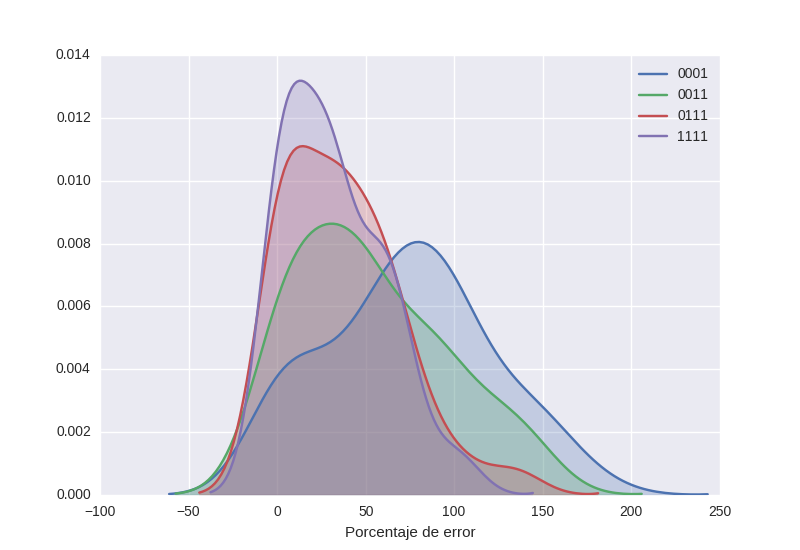
\includegraphics[width=\textwidth]{img/ejercicio3/exp3_distribuciones.png}
%    \caption{Distribución de los porcentajes de error sobre casos con solución válida.}
%    \label{fig: ej3_exp3_an1_distr_validados}
%  \end{center}
%\end{figure}

En esta sección vamos a ir mostrando y explicando los resultados de cada experimento que propusimos.
En resumen vamos a ir variando cada una de las variables e ir comparando tiempos con respecto a cada una de ellas, es decir, vamos a ir variando; capacidad de mochila, cantidad de paradas y cantidad de gimnasios.

\subsubsection{Experimento 1: Cantidad de Gimnasios vs Tiempos de ejecución}

En el siguiente gráfico fijamos la mochila y variamos la cantidad de gimnasios, sin usar escala logarítmica:

\begin{itemize}
\item Cantidad de paradas = 100.
\item Capacidad mochila = 20.
\item La cantidad de pociones necesarias en cada gimnasio es random.
\end{itemize}


\begin{figure}[H]
  \begin{center}
    \begin{subfigure}[b]{0.70\textwidth}	
        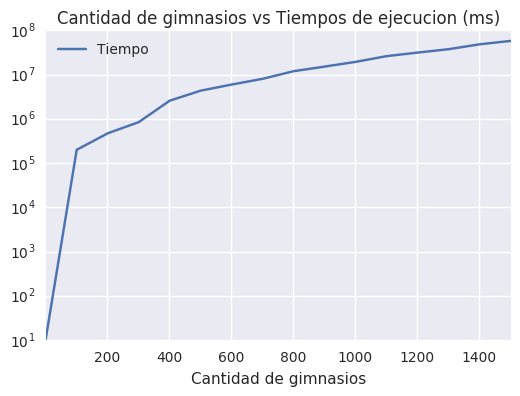
\includegraphics[width=\textwidth]{img/ejercicio2/losPosta/grafico_gimnasios.png}
        \caption{Gráfico variando cantidad de gimnasios.}
        \label{fig: ejercicio1_ejemplo_camino1_2}
    \end{subfigure}
  \end{center}
\end{figure}


Podemos ver como se comportan los tiempos a medida que vamos aumentando la cantidad de gimnasios, en si los valores no son tan importantes.
Ya que a la larga deberia ser el mismo crecimiento, por como se comporta nuestro algoritmo, es decir, sabemos que siempre va a ir a buscar una parada más cerca y
en caso de poseer suficientes posiciones para atacar un gimnasio, lo hace. Por más que tengamos una amplia mochila o tengamos muchas pokeparadas, lo que importa es la cantidad de gimnasios y
la cantidad de pociones que necesitamos para atacarlo. Si tenemos gimnasios con el requisito de posiciones en valores altos, el tiempo va a ser mayor ya que va a requerir de recorrer más nodos para poder derrotarlos.
Lo interesante del gráfico es su semejanza a una funcion logaritimica. No sabemos exactamente porque de este comportaminto, pero nos dios la 
sensacion de que en funcion de los gimnasios solamente el algoritmo, a la larga, tiene tiempos logartimos en funcion de los gimnasios.


\subsubsection{Experimento 2: Cantidad de paradas vs Tiempos de ejecución}

\begin{itemize}
\item Cantidad Gimnasios = 50.
\item Capacidad de la mochila = 200.
\item La cantidad de pociones necesarias en cada gimnasio es random.
\end{itemize}

Esta vez vamos a mostrar como se comporta nuestro algoritmo en terminos de tiempo al aumentar la cantidad de paradas y dejar fija la capacidad de la mochila y la cantidad de gimnasios:

\begin{figure}[H]
  \begin{center}
    \begin{subfigure}[b]{0.70\textwidth}
        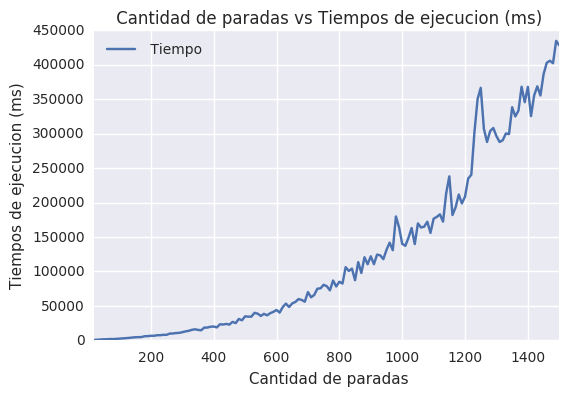
\includegraphics[width=\textwidth]{img/ejercicio2/losPosta/grafico_sin_logs.png}
        \caption{Gráfico variando la cantidad de paradas.}
        \label{fig: ejercicio1_ejemplo_camino1_2}
   \end{subfigure}
  \end{center}
\end{figure}


El mismo gráfico con escala logartimica en el eje y:
\begin{figure}[H]
  \begin{center}
    \begin{subfigure}[b]{0.70\textwidth}
        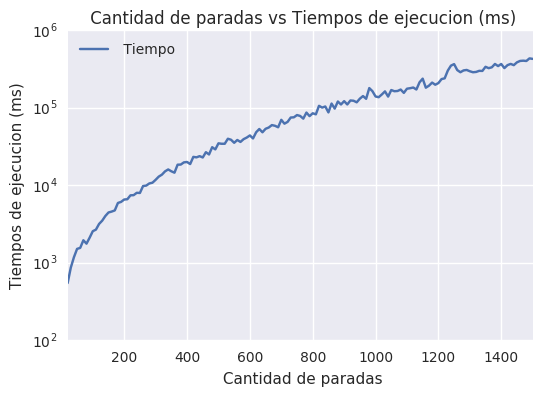
\includegraphics[width=\textwidth]{img/ejercicio2/losPosta/grafico_log_y.png}
        \caption{Grafico variando la cantidad de paradas escala logarimica en eje y.}
        \label{fig: ejercicio1_ejemplo_camino1_2}
   \end{subfigure}
  \end{center}
\end{figure}

Y por último el mismo grafico pero aplicando la escala en ambos ejes:

\begin{figure}[H]
  \begin{center}
   \begin{subfigure}[b]{0.70\textwidth}	
        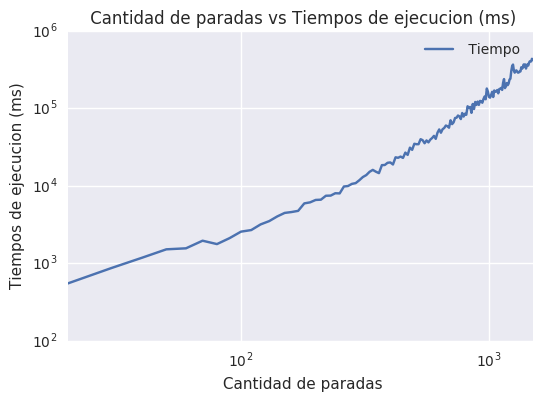
\includegraphics[width=\textwidth]{img/ejercicio2/losPosta/grafico_con_2_logs.png}
        \caption{Grafico variando la cantidad de paradas escala logarimica en x e y.}
        \label{fig: ejercicio1_ejemplo_camino1_2}
   \end{subfigure}
  \end{center}
\end{figure}

En estos gráficos podemos ver como se comporta nuestro algoritmo cuando fijamos la cantidad de gimnasios y la capacidad de la mochila, y variamos la cantidad de paradas en funcion del tiempo.
Podemos observar que a medida qeu las paradas son mayores, las corridas son más largas haciendo que el tiempo aumente de forma exponencial.
Esto igualmente tiene muchas varibles, pero en nuestro caso al aumentar la cantidad de pokeparadas, estamos aumentando los tiempso de ejecucion ya que, cada vez que querramos visitar el proximo nodo
vamos a necesitar saber las distancias de todos los nodos con respecto al que estamos parados, haciendo que la complejidad temporal suba considerablemente.

\subsubsection{Experimento 3: Capacidad de la mochila vs Tiempos de ejecución}

Nos queda por mostrar como varian los tiempos al variar la capacidad de la mochila y dejar fijos ambos valores de paradas y gimnasios:

\begin{itemize}
\item Cantidad de Gimnasios = 50.
\item Cantidad de pokeparadas = 100.
\end{itemize}

\begin{figure}[H]
  \begin{center}	
    \begin{subfigure}[b]{0.70\textwidth}
        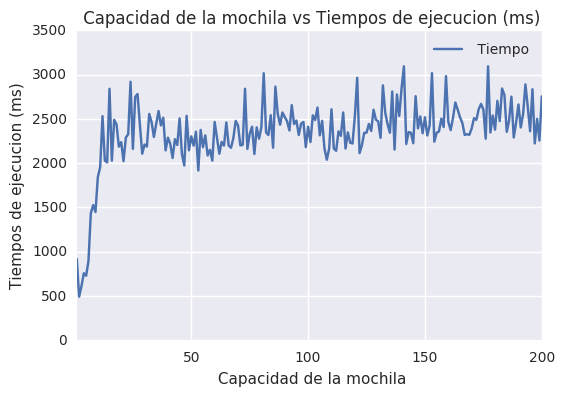
\includegraphics[width=\textwidth]{img/ejercicio2/losPosta/grafico.png}
        \caption{Gráfico variando la capacidad de la mochila.}
        \label{fig: ejercicio1_ejemplo_camino1_2}
 \end{subfigure}
  \end{center}
\end{figure}

En este gráfico vemos como se comporta el goloso al variar la capacidad de la mochila y dejar fija la cantidad de pokeparadas y gimnasios.
Como se observa el comportambien es parecido por más que aumentemos la capacidad de la mochila, creemos que esto tiene bastante sentido ya que
aumentar la capacidad solo hace que pueda llevar más posiones, pero por como actua nuestro goloso, si en algun momento tiene las suficientes posiones como para ir a 
derrotar un gimnasio, lo va a ir a hacer. Entonces lo que permite esto es no aprovechar cantidades muy grandes de capacidad de mochila, ya que igualmente (si a priori puede) va a ir al gimnasio con menor
requisito de pociones. Luego el gráfico no debería variar demasiado entre instancias distintas de este tipo.

\subsubsection{Experimento 4: Cantidad de Gimnasios vs Tiempos de ejecución TSP}

Ahora mostramos el caso tsp fijando mochila y paradas, pero variando la cantidad de gimnasios.

\begin{itemize}
\item Cantidad de paradas = 100.
\item Capacidad de la mochila = 20.
\item La cantidad de pociones necesarias en cada gimnasio es random.
\end{itemize}

\begin{figure}[H]
  \begin{center}	
    \begin{subfigure}[b]{0.49\textwidth}
        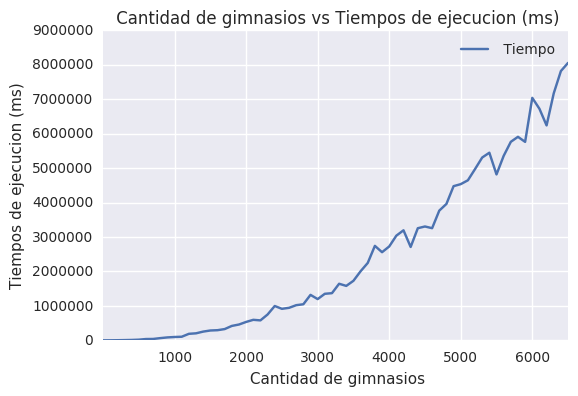
\includegraphics[width=\textwidth]{img/ejercicio2/losPosta/grafico_sin_log.png}
        \caption{Gráfico variando las mochilas.}
        \label{fig: ejercicio1_ejemplo_camino1_2}
 \end{subfigure}
 
    \begin{subfigure}[b]{0.49\textwidth}
        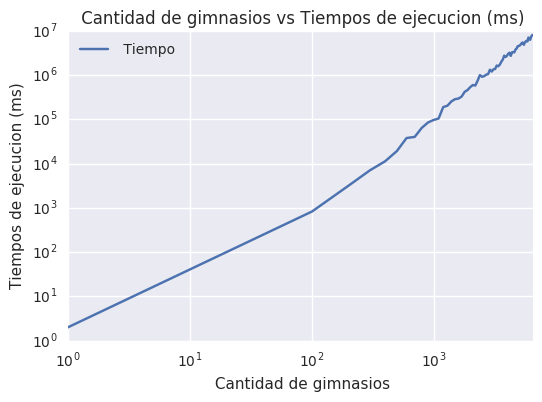
\includegraphics[width=\textwidth]{img/ejercicio2/losPosta/grafico_2log.png}
        \caption{Gráfico variando la cantidad de gimnasios con escala logarimica en x e y.}
        \label{fig: ejercicio1_ejemplo_camino1_2}
  \end{subfigure}

  \end{center}
\end{figure}
 	  
\begin{figure}[H] 
 \begin{center}
	\begin{subfigure}[b]{0.59\textwidth}
        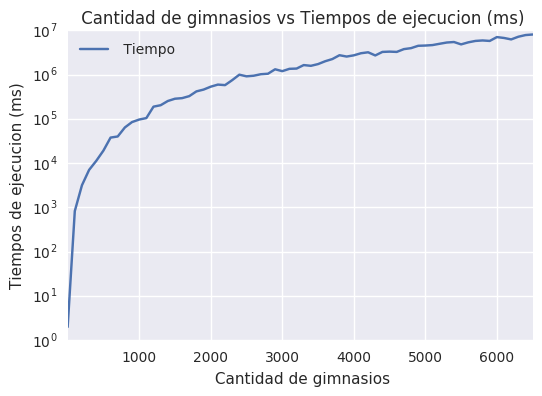
\includegraphics[width=\textwidth]{img/ejercicio2/losPosta/grafico_logy.png}
        \caption{Gráfico variando la cantidad de mochilas con escala logaritmica en eje y.}
        \label{fig: ejercicio1_ejemplo_camino1_2}
 \end{subfigure}
  \end{center}
\end{figure}

Este gráfico muestra el rendimiento del goloso con tsp, podemos observa con relación al primer gráfico que mostramos en esta sección.
que su crecimento a medida que vamos aumentando los gimnasios es de tipo exponencial.

\subsubsection{Experimento 5: Comparacion entre los tiempos vs complejidad ($n^2$) y ($n^3$) }

\begin{figure}[H]
  \begin{center}	
    \begin{subfigure}[b]{0.60\textwidth}
        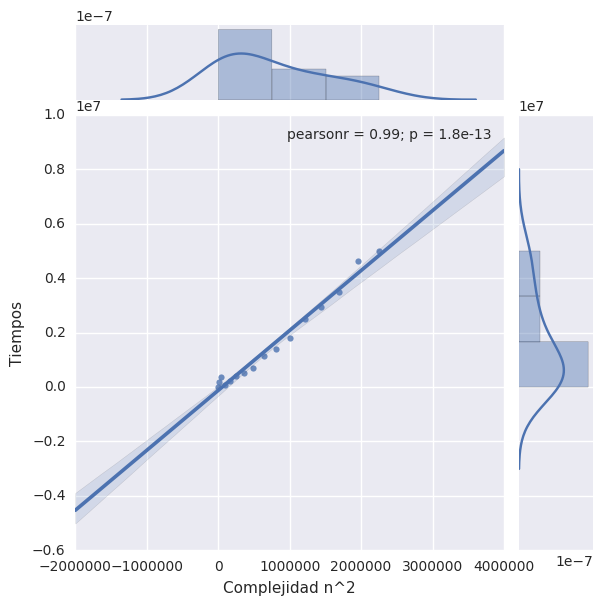
\includegraphics[width=\textwidth]{img/ejercicio2/losPosta/pearsonncuadrado.png}
        \caption{Gráfico variando las mochilas.}
        \label{fig: ejercicio1_ejemplo_camino1_2}
 \end{subfigure}
 
    \begin{subfigure}[b]{0.60\textwidth}
        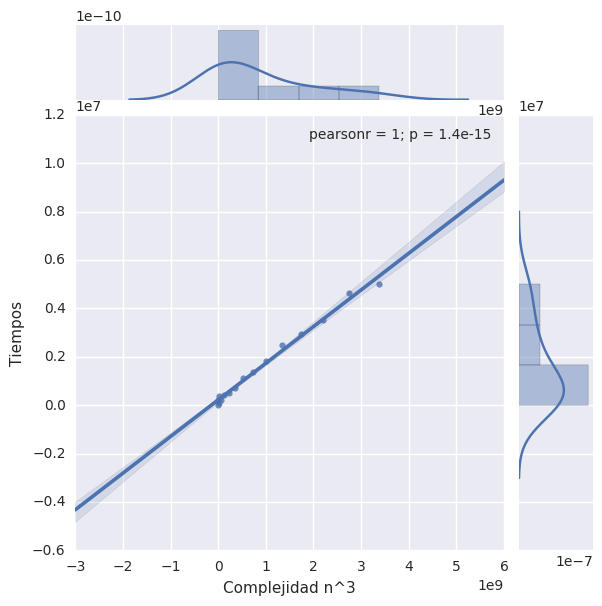
\includegraphics[width=\textwidth]{img/ejercicio2/losPosta/pearsonncubo.png}
        \caption{Gráfico variando la cantidad de gimnasios con escala logarimica en x e y.}
        \label{fig: ejercicio1_ejemplo_camino1_2}
	   \end{subfigure}

  \end{center}
\end{figure}

En el gr\'afico se puede ver una muy buena correlaci\'on entre los tiempos obtenidos en las corridas y una funci\'on cuadr\'atica. Esta observaci\'on la pudimos realizar debido a que el coeficiente de Pearson es 0.99 y su $valor p$ es muy pequeño. De esta manera podemos afirmar que nuestra cota de complejidad estaba bien calculada.


\subsubsection{Experimento 6: Evaluacion de calidad de la solucion con porcentaje de error }

\begin{figure}[H]
  \begin{center}	
    \begin{subfigure}[b]{0.60\textwidth}
        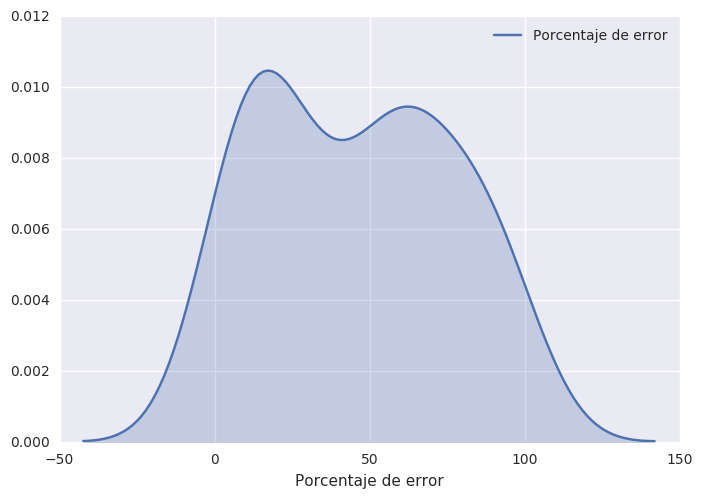
\includegraphics[width=\textwidth]{img/ejercicio2/losPosta/grafico_distribucion.png}
        \caption{Comparacion de calida de la solucion.}
        \label{fig: ejercicio1_ejemplo_camino1_2}
    \end{subfigure}
  \end{center}
\end{figure}

En la figura podemos observar que el error del algoritmo suele variar m\'as que nada entre 25\% y el 75\% de la soluci\'on exacta. Este resultado nos va a servir como cota superior del error de los resultados de la heur\'istica y la metaheur\'istica.